\documentclass[12pt,a4paper]{report}
\usepackage[utf8]{inputenc}
\usepackage[portuguese]{babel}
\usepackage[T1]{fontenc}
\usepackage{amsmath}
\usepackage{amsfonts}
\usepackage{amssymb}
\usepackage{graphicx}
\usepackage{fourier}
\usepackage[left=2cm,right=2cm,top=2cm,bottom=2cm]{geometry}
\author{Luiz Guilherme - Professor de Matemática}
\title{Matemática para Concursos Públicos}
\date{Última atualização:  \today \\ \qrcode{https://docs.google.com/viewer?url=https://raw.githubusercontent.com/lgfpcampos/Concursos/main/apostila.pdf}} 
\usepackage{tikz}
\usepackage{tcolorbox}
\usepackage{hyperref}
\usepackage{qrcode}
\usepackage{xcolor}
\usepackage{fontawesome}
\usepackage{enumerate}
\usepackage[Bjornstrup]{fncychap}
\usepackage{multicol}

\begin{document}

\newcommand{\quest}[4]{ \item 
	\textbf{#1} {\color{red}\faYoutubePlay}\\ % Banca e Concurso
	 {#2}\\ %enunciado
		\begin{minipage}{12cm}
		\begin{enumerate}
			{#3} %alternativas
		\end{enumerate}
	\end{minipage}
	\qrcode{#4&list=UULFeA_dOOqAA4DB92B_BWDU7Q}} %youtube


\maketitle
\tableofcontents	

\begin{enumerate}
\chapter{Máximo Divisor Comum e Mínimo Múltiplo Comum}

\quest{Oficial de Justiça 2023 - VUNESP}{Uma empresa executa serviços aos seus clientes somente de segunda-feira a sexta-feira, independentemente de haver feriado ou não. Para seu cliente X&W, ela executa serviços a cada 12 dias, excluindo-se sábados e domingos, enquanto que para seu cliente W&Z, ela executa serviços a cada 33 dias, também excluindo-se sábados e domingos. No dia 15 de agosto de 2023, uma terça-feira, essa empresa executou serviços para ambos os clientes.
Isso significa que a vez imediatamente posterior em que ela executou os serviços para ambos os clientes, em um mesmo dia, foi uma}
{\item sexta-feira.
\item segunda-feira.
\item quinta-feira.
\item quarta-feira.
\item terça-feira.}
{https://youtu.be/o07aeZ4jtj4}
\chapter{Média Aritmética Simples e Ponderada}

\quest{Oficial de Justiça 2023 - VUNESP}{O gráfico apresenta o número de acertos na prova de Língua Portuguesa e de Matemática, aplicada a dois candidatos, A e B, em um concurso interno para promoção de cargo:\\
	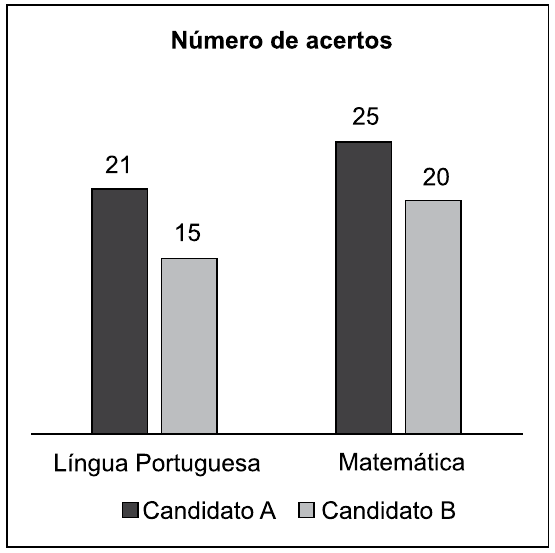
\includegraphics[scale=.5]{fig001.png}\\
Sabendo-se que a prova de Língua Portuguesa tinha 	peso 2 e a de Matemática tinha peso 3 para o cargo em 	concurso, que cada uma das provas tinha 50 questões, 	e que a nota de cada prova é igual ao número de acertos correspondente, é correto afirmar que o número de questões de Matemática que o candidato B deveria ter acertado a mais, para que a média aritmética ponderada das notas das suas provas fosse igual à média aritmética ponderada das notas das provas do candidato A, é igual a}
{\item 9.
\item 20.
\item 10.
\item 29.
\item 27.}
{https://youtu.be/BvsQZctqarQ}

\chapter{Razão e Proporção}
\quest{Oficial de Justiça 2023 - VUNESP}{No ano de 2022, 3 em cada 8 edifícios comercializados em determinada região foram adquiridos pelo empreendimento A&B, que investiu R\$ 1,35 bilhão na compra desses edifícios, ao preço médio de R\$ 15 milhões cada edifício. Dos edifícios não adquiridos pelo empreendimento A&B e que foram comercializados naquela r­egião, o empreendimento R&T adquiriu metade, ao custo total R\$ 1,23 bilhão, o que fez com que o preço médio, por edifício adquirido pela R&T, fosse de}
{
\item R\$ 16,3 milhões.
\item R\$ 16,1 milhões.
\item R\$ 16,5 milhões.
\item R\$ 16,4 milhões.
\item R\$ 16,2 milhões.}
{https://youtu.be/41SHCi5jX54} 

\quest{Técnico Interno BBTS 2023 - FGV}{Oscar, na primeira metade de uma partida de basquete, acertou 12 de 16 arremessos e, na segunda metade, acertou os 8 arremessos que fez. Jordan, por sua vez, fez 12 arremessos na primeira metade do jogo e 18 arremessos na segunda metade. Em cada metade do jogo, o percentual de acertos de Oscar foi maior do que o percentual de acertos de Jordan. Entretanto, ao final do jogo, os percentuais de acerto totais dos dois jogadores foi o mesmo. Na segunda metade do jogo, o número de acertos que Jordan teve a mais do que o seu número de acertos na primeira metade foi}{
\item 9.
\item 10.
\item 11.
\item 12.
\item 13.}
{https://youtu.be/jgkJfktwl98}

\chapter{Regra de Três Simples e Composta}

\quest{Oficial de Justiça 2023 - VUNESP}
{Considere as informações apresentadas na tabela a seguir, relacionadas à produção de certa peça que é
realizada apenas por máquinas iguais, trabalhando ao mesmo tempo, com a mesma capacidade de produção.\\
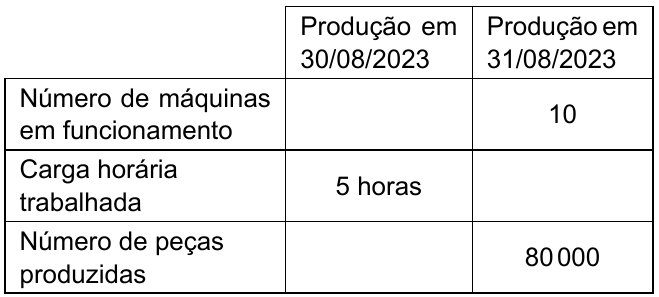
\includegraphics[scale=.5]{fig002.png}\\
Sabendo-se que as informações apresentadas são proporcionais, que em 30/08/2023 o número de máquinas
em funcionamento era um quinto maior que o número de máquinas trabalhando no dia seguinte, e que o número
de peças produzidas em 31/08/2023 foi quatro terços do número de peças produzidas no dia anterior, é correto afirmar que a carga horária trabalhada no dia 31/08/2023 foi de}
{\item 8 horas.
\item 7 horas.
\item 9 horas.
\item 8 horas e 30 minutos.
\item 7 horas e 30 minutos.}
{https://youtu.be/mVp0Bf8s8J4}

\end{enumerate}



\end{document}